\documentclass[conference]{IEEEtran}
\IEEEoverridecommandlockouts
% The preceding line is only needed to identify funding in the first footnote. If that is unneeded, please comment it out.
\usepackage{cite}
\usepackage{amsmath,amssymb,amsfonts}
\usepackage{algorithmic}
\usepackage{graphicx}
\usepackage{textcomp}
\usepackage{xcolor}
\def\BibTeX{{\rm B\kern-.05em{\sc i\kern-.025em b}\kern-.08em
    T\kern-.1667em\lower.7ex\hbox{E}\kern-.125emX}}
\begin{document}

\title{Comparison of two selected ML models for predicting deaths due to COVID-19 outbreak}

\author{\IEEEauthorblockN{1\textsuperscript{st} Szymon Krasuski}
\IEEEauthorblockA{\textit{Warsaw University of Technology} \\
Warsaw
}
\and
\IEEEauthorblockN{2\textsuperscript{nd} Janusz Mikłuszka}
\IEEEauthorblockA{\textit{Warsaw University of Technology} \\
Czeladź
}
}


\maketitle

\begin{abstract}
\dots
\end{abstract}

\begin{IEEEkeywords}
COVID-19, Machine learning, Autoregression.
\end{IEEEkeywords}

\section{Introduction}
Current coronavirus pandemic started in chinese Wuhan, in December 2019. On 11 March WHO made the assessment that COVID-19 can be
 characterized as pandemic which became global problem. On 4 March first case in Poland appeared. From this time number of confirmed cases was steadily increasing.
 Month later there was 5000 confirmed cases.

\dots

\section{Problem Description}
Using databases of confirmed cases, death cases and recovered cases of COVID-19 we can create model which can give us predictions of future cases.
 Based on these prediction decisions can be made regarding public restrictions and other regulations.
% może jakieś wykresy wzrostu dać czy co innego

\dots

\section{Domain Implementation}
% tego nie jestem pewien co powinno być, może coś w czym robimy
We are using Python enviroment to create application which based on provided data and prediction horizon, makes predictions of number of deaths per day.
 We primarily uses autoregressive (AR) models which are primarily used to describe time-varying processes in nature. This type of model specifies the output
  variable based on its previous values and stochastic term. Along with moving-average (MA) model it is component of more general autoregressive-moving-average
  model (ARMA). Dynamic of the autoregressive model of order p AR(p) is given by:
\begin{equation}
    X_t = c + \sum_{i=1}^{p} (\phi_iX_{t-i}) + \epsilon_t
\end{equation}
where
p - order of the model\newline
$ \phi $ - parameters of the model\newline
c - constant\newline
$\epsilon_t$ - white noise\newline


Moving average model of order q MA(q) is written:
\begin{equation}
    X_t = \mu + \epsilon_t + \sum_{i=1}^{q} (\theta_i\epsilon_{t-i})
\end{equation}

ARMA(p,q) notation refers to AR(p) and MA(q) models:
\begin{equation}
    X_t = c + \epsilon_t +\sum_{i=1}^{p} (\phi_iX_{t-i}) + \sum_{i=1}^{q} (\theta_i\epsilon_{t-i})
\end{equation}


Project structure is organised into consistent class which implements methods for gathering data, training machine learning model and data visualization.
\newline
\newline
Data gathering is separate module that allows to download data in the runtime from provided web server or load data from local file.
Data format has to be consistent with format provided by user dtandev in repository "coronavirus" published on GitHub platform.
Data is presented as summarized numbers per columns starting from 3rd March 2020.
Because of that data gathering module on reading raw data has additonal steps which
\begin{itemize}
\item Based on data in columns 'Deaths' counted are 'Day-to-day Deaths' in order to normalize training data to not have only incrementing trend.
\item Based on data of 'Confirmed' minus values from 'Deaths' and 'Recovered' is computed data of currently sick people in Poland.
\end{itemize}
Complete data is returned in Pandas DataFrame.
\newline
\newline
Main class contain methods which implement steps easy to split for external resources e.g. GUI applications:
\begin{itemize}
\item \textit{load\_data} - implements data gathering model to load data from web or local file. It is possible to provide data also as complete DataFrame during object initialization.
\item \textit{set\_predict\_horizon} - sets data up to which next data points should be predicted. Data should be datatime object from datatime library.
\item \textit{train\_AR} - method which trains Autoregression model based on previously loaded data.
\item \textit{train\_MA} - method which trains Autoregressive Integrated Moving Average model based on previously loaded data.
\item \textit{predict} - Because it is possible to alternatively train model with two separate methods then this method uses one of models (the one that was run as last) and predicts next data points up to predict horizon.
\item \textit{plt} - this method prints out matplotlib plot with actual data and predicted data points.
\item \textit{get\_dcc\_Graph} - this method returns Dash Core Components Graph with actual data and predicted data which may be used with GUI applications created in Dash
\end{itemize}
Presented project utilizes Dash library in order to implement user-friendly application.
\begin{figure}[h!]
    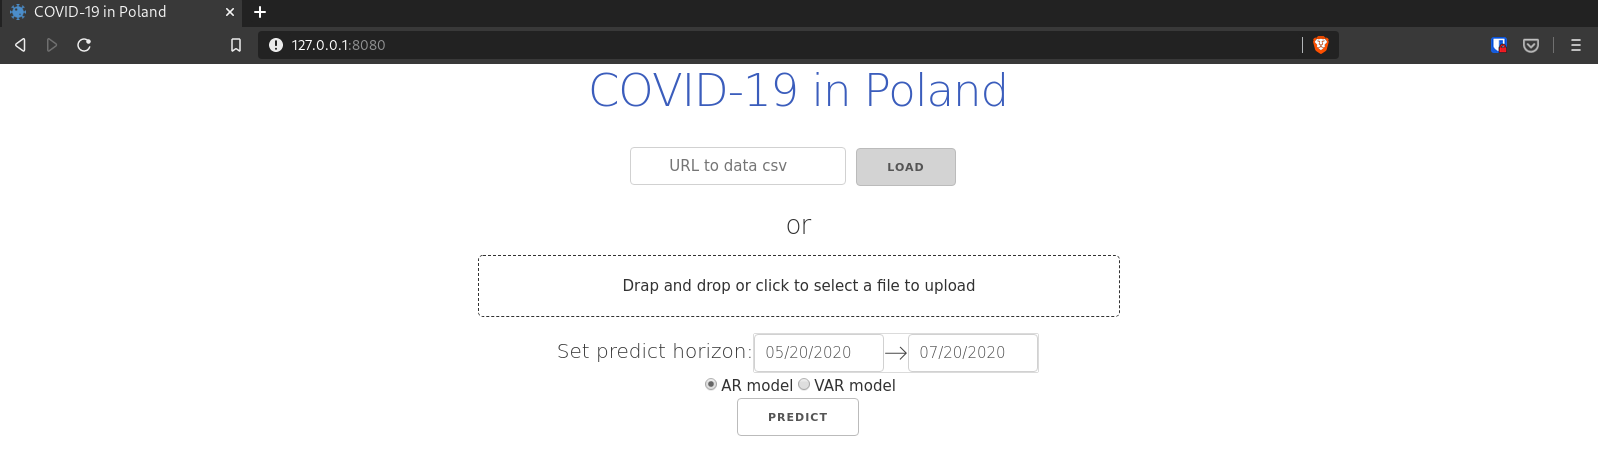
\includegraphics[width=\linewidth]{images/gui1.png}
    \caption{User welcome screen}
    \label{fig:gui1}
\end{figure}
\newline
User at the first site layout have simple control which allow to load data from pasted URL (by default URL to data from dtandev/coronavirus repository is available to choose from text field) or local file.
Afterwards, user has possiblity to set data which will be used as predict horizon adn finally choose one of two training models.
\newline
When user clicks 'Predict' button then below is generated interactive Dash Core Component Graph.
\begin{figure}[h!]
    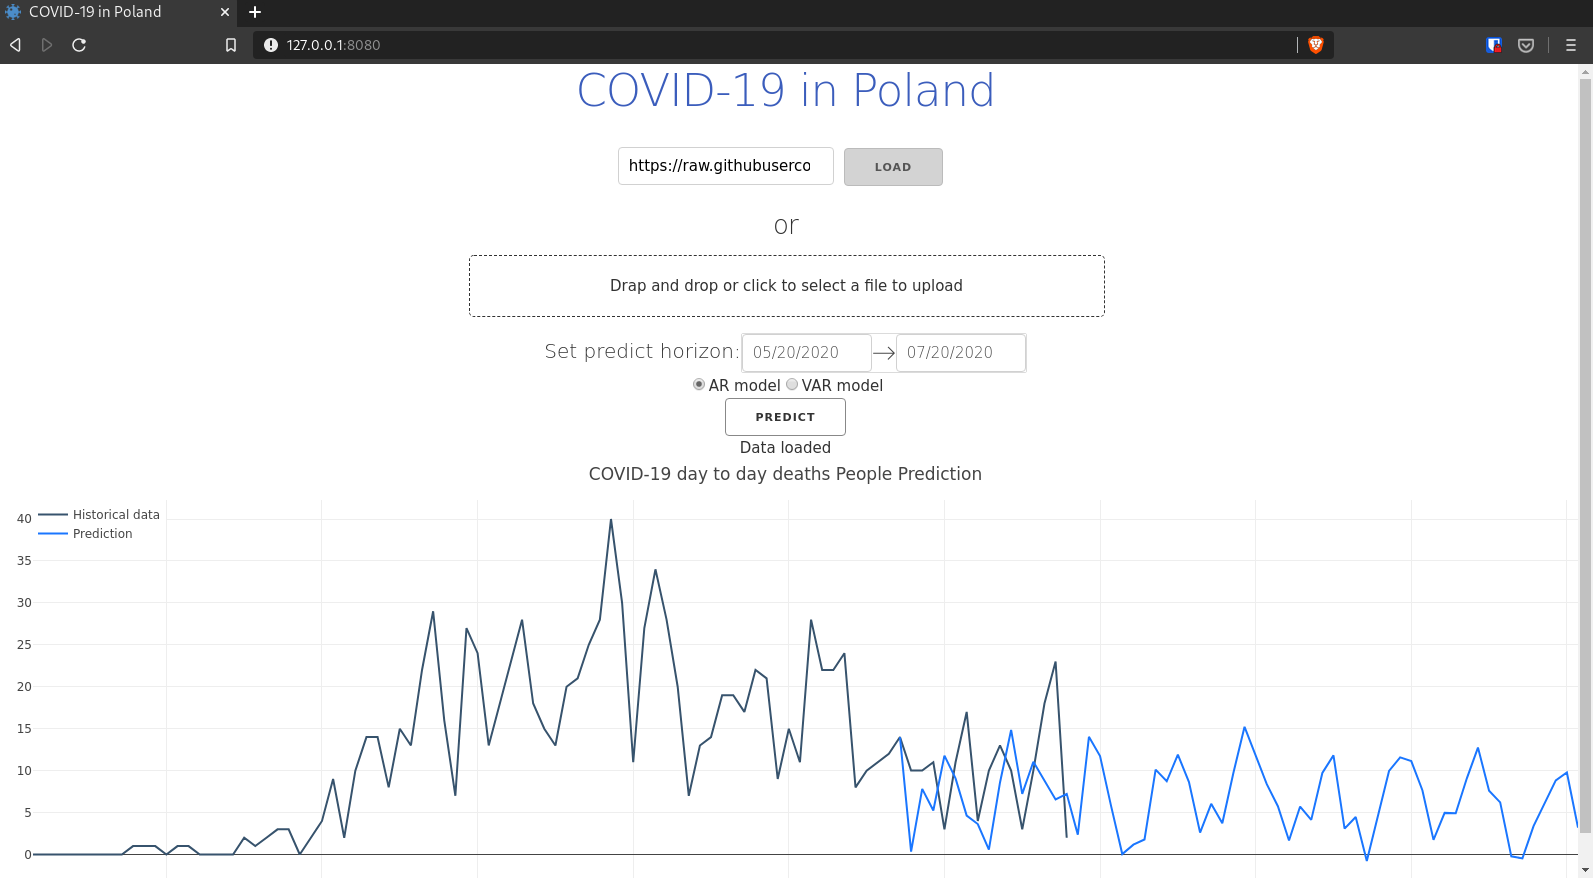
\includegraphics[width=\linewidth]{images/gui2.png}
    \caption{Application after setting parameters and prediction process}
    \label{fig:gui2}
\end{figure}
\newline
User has always possiblity to modify parameters and repeat prediction from any point of process.

\section{Machine Learning Models}
We are using AutoReg function from statsmodel library. This function uses Autoregressive. It uses only vector of values we want to predict.
 We also need to define order of the model.
\dots

\section{Results}
\dots

\section{Summary}
\dots


\begin{thebibliography}{00}
\bibitem{b1} https://www.sciencedirect.com/science/article/pii/0047259X85900272
\bibitem{b2} https://link.springer.com/chapter/10.1007/978-1-4612-1694-0\_12
\bibitem{b3} https://journals.ametsoc.org/doi/full/10.1175/JHM517.1
\bibitem{b4} https://github.com/dtandev/coronavirus
\bibitem{b5}
\bibitem{b6}
\bibitem{b7}
\end{thebibliography}
\vspace{12pt}

\end{document}
